
\newcommand{\lib}[1]{{\normalfont\textsf{#1}}}
\newcommand{\EBImage}{{\normalfont\textsf{EBImage}}}

\title{Automated image analysis for microscopy screens with EBImage}
\author{by Oleg Sklyar and Wolfgang Huber}

\maketitle

With recent advances in microscopy, genome-wide phenotypic microscopy screens have become technically feasible \citep{R:Neumann:2006}. While generally providing a higher information content than other high-throughput experiments, such screens introduce additional challenges in data analysis. Image processing and image analysis need to be performed in order to extract experiment-specific image descriptors from raw images that can be further analyzed statisticaly. Because thousands of images have to be analyzed in the same or similar manner, these steps need to be automated as well.

Many microscope manufacturers provide software that is not intended for automated analysis of thousands of images. Support for statistical analysis of image descriptors is usually missing as well.

We present \EBImage\ - a {\em BioConductor} package designed to combine algorithms for image processing and analysis with the power of \R{} in statistical computing.

The package initially aimed to support automated image analysis in genome-wide cell-based RNA interference (RNAi) microscopy screens \citep{R:Fuchs+Boutros:2006}. Cellular and nuclear size, density and luminescent intensity are the most important image descriptors in this case. Until now, \lib{CellProfiler} \citep{R:Carpenter:prep} was the only publically avaliable package that could deal with the automated extraction of image descriptors from images of cells and nuclei. Alternatively, researchers were writing in-house analysis software geenerally not available in public domain \citep{R:Neumann:2006}.

Although designed for the analysis of cell-based screens, \EBImage\ is not limited to these particular types of images or image descriptors. It provides algorithms and tools for general handling of images in \R{}, as well as ways to process and analyze arbitrary images in many graphic formats.

\section*{Handling images}

\EBImage\ is aimed to work primarily with grayscale images. However, many high-level image processing routines support colored images in the RGB mode as well. This support is built-in to enable the initial preprocessing of images and to enhance displaying of the analysis results. Most of the analysis routines require grayscale data though.

Images in \EBImage\ are stored in objects of class \code{Image}, which is directly inherited from {\tt array}. Data are always stored as 3D arrays with the third dimension being 1 for 2D images. At the moment, the only additional field in \code{Image} is \code{rgb}, a logical value defining the color mode. It also determines the internal numeric format of the data: a 4-byte integer for RGB's and double for grayscales. Many analysis routines will assume grayscale data in the range {\tt [0..1]}, but there are no formal limits for the range.

Because of the nature of this data storage, RGB data are generally useless for any direct analysis. However, the fact that \code{Image} is inherited from \code{array} enables a direct application of all \R{} functions that work with arrays to grayscale images. This includes mathematical routines, histograms, subsetting etc. For example, the sharpened image in Figure \ref{figure:sharpening}{\bf c} can be obtained using a naive version of the {\em unsharp-mask} filter implemented as a simple subtraction of the median (Figure \ref{figure:sharpening}{\bf b}) from the source image in Figure \ref{figure:sharpening}{\bf a}. The source image here, which is a subset of the original microscopic image, is first lightened by applying the {\em square root} function:

\begin{verbatim}
> a <- origImage[150:300, 180:330, 1]
> b <- medianFilter(a, 40)
> c <- normalize(sqrt(a) - b)
\end{verbatim}

\begin{figure}
\vspace*{.1in}
\begin{center}
\scalebox{1.1}{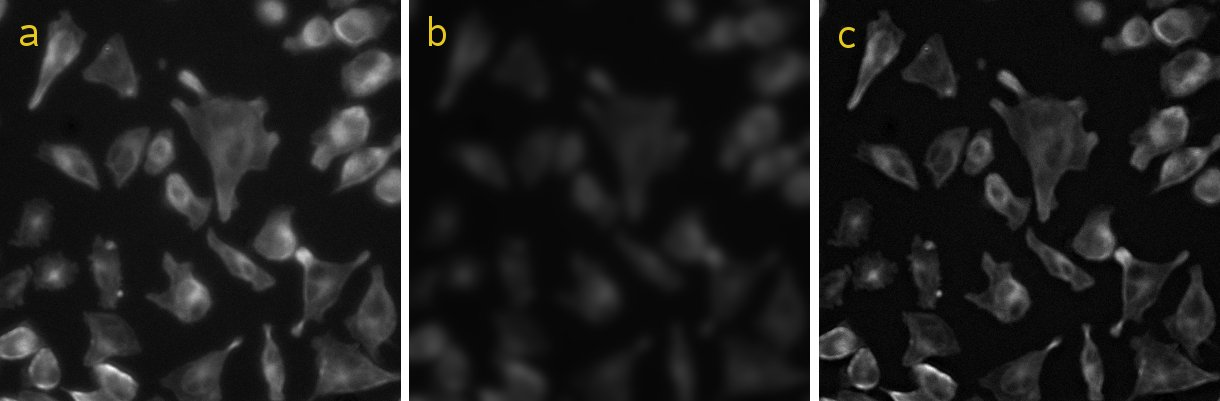
\includegraphics{sharpen.jpg}}
\end{center}
\caption{\label{figure:sharpening}
    Implementation of the simple {\em unsharp-mask} filter: (a) source image, (b) adaptive median, (c) sharpened image after normalization
}
\end{figure}

\EBImage\ uses {\em Magick++} interface to \lib{ImageMagick} image processing library \citep{R:ImageMagick:1999} for many high-level routines including input-output operations. \lib{ImageMagick} supports over 95 image formats including formats like JPEG, TIFF and PNG relevant for microscopy. \EBImage\ can read-write multipage images or process multiple files simultaneously. For example, to read all colored PNG files in the current directory into a single object of class \code{Image} and save them afterwards in the grayscale mode as a single multipage TIFF file, the following code can be used:

\begin{verbatim}
> files <- dir(pattern = ".png")
> im <- read.image(files, rgb = TRUE)
> img <- toGray(im)
> write.image(img, "single_multipage.tif")
\end{verbatim}

Currently \EBImage\ is the only \R{} package that allows for reading data of images in such a number of formats into \R{}. Beside operations on local image files, HTTP and FTP network protocols are supported by \EBImage. The package can read from both, HTTP and anonymous FTP, and it can write to anonymous FTP only.

New images can also be easily created; image data can then be assigned using subscripts. For example, the following code generates a single 2D grayscale image of 100x100 pixels with black and white vertical stripes:

\begin{verbatim}
> im <- Image(0, c(100,100))
> im[c(1:20, 41:60, 81:100),,] = 1
\end{verbatim}

\section*{General image processing}

One part of the \EBImage\ functionality is to provide an \R{}-interface to \lib{ImageMagick} image processing routines (or filters). At the moment, \EBImage\ does not port all possible \lib{ImageMagick} routines to \R{}, but aims for those that are relevant for preprocessing and enhancing images from microscopy. Other filters that do not come with \lib{ImageMagick} are implemented directly in \EBImage.

Image filters in \EBImage\ are implemented as functions acting on objects of class \code{Image} and returning new mofified images of the same size (excluding transformation filters). One can generally divide available filters into four categories: image {\em enhancement}, image {\em segmentation}, image {\em transformation} and {\em color correction}. The most important filters are listed below. Some of them should be known to the reader from the {\em interactive} graphics packages like \lib{The GIMP} or \lib{Adobe Photoshop}:

\begin{itemize}
    \setlength{\itemsep}{0in}
    \item \code{sharpen} and \code{unsharpMask} generate a sharpened version of the original image. In the code to Figure \ref{figure:sharpening}, a simplified implementation of the {\em unsharp-mask} filter was shown, demonstrating the idea behind this filter
    \item \code{reduceNoise} reduces image noise by blurring small noise clusters into the surrounding color
    \item \code{gaussFilter} - this filter performs gaussian blur on the original image softening sharp edges and noise
    \item \code{thresh} is the \EBImage\ implementation of the {\em adaptive threshold} filter. It uses a moving frame of a specified size to generate a binary black-and-white image using the mean of the original grayscale image within the frame as the base for thresholding
    \item \code{distMap} generates a {\em Euclidian Distance Transform} (distance map) of the original grayscale image using algorithm by \citep{R:Lotufo+Zampirolli:2001}. On a distance map, values of pixels indicate how far those are removed from the nearest background (black). The implementation is adapted from the \lib{ANIMAL} library, currently a part of the \lib{SIP toolbox} \citep{R:SIP:2005}
    \item \code{normalize} scales grayscale image data to the specified range, normally \code{[0..1]}; for RGB's this filter stretches image pallete to reach the maximum possible brightness while keeping the ratios of color channels (RGB)
    \item \code{sample.image} resizes images proportionally using subpixel sampling algorithms
\end{itemize}

\EBImage\ provides a group of functions to convert images between RGB and grayscale and to work with individual color channels of RGB's. Because for RGB images, different color channels reside in different parts of the internal 4-byte representation, color channels are additive as in the example below. However, if any particular color exceeds its maximum range, this may affect other colors.

The following code demonstrates how typical miscroscopy images recorded in 3 different color channels as grayscales (Figure \ref{figure:channels} {\bf a}, {\bf b} and {\bf c}) can be put together into one {\em false-color} representation (Figure \ref{figure:channels} {\bf d}); or alternatively, a single false-color image can be decomposed into individual channels:

\begin{verbatim}
> files <- c("ch1.png","ch2.png","ch3.png")
> abc <- read.image(files)
> a <- toGreen(abc[,,1])
> b <- toRed(abc[,,2])
> d <- a + b + toBlue(abc[,,3])
> C <- getBlue(d)
\end{verbatim}

\begin{figure}
\vspace*{.1in}
\begin{center}
\scalebox{1.0}{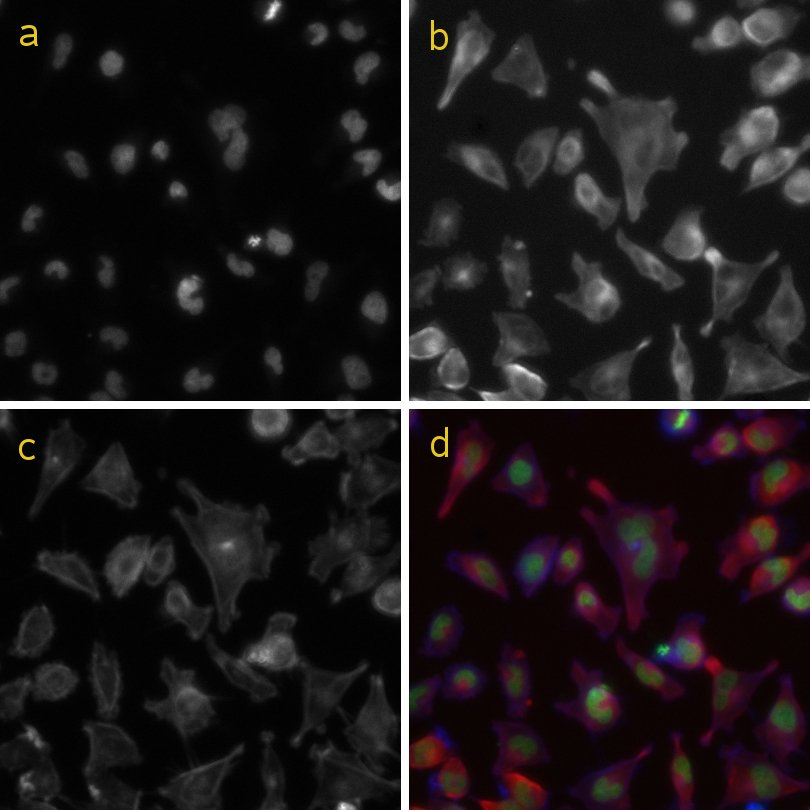
\includegraphics{channels.jpg}}
\end{center}
\caption{\label{figure:channels}
    Composition of a false-color image (d) from a set of microscopy images recorded in 3 different color channels as grayscales (a, b and c)
}
\end{figure}

Images can be displayed in two different ways. \EBImage\ defines method \code{display} that displays images in an interactive X11 window, in which multiple images can be animated and browsed. This function is very fast, but (so far) it fails on some systems (including all tested \lib{MacOS X} and some \code{ssh -X} sessions). It does not use \R{} graphic devices and, thus, cannot be redirected to any of those. As a workaround, for grayscale images \EBImage\ provides method \code{plot.image}, which is a wrapper around standard \R{} \code{image} function. \code{plot.image} uses \R{} graphic devices. The function is very slow (which is defined by \code{image}) and it plots only the first image of any 3D stack. In the following example, the first command provides possibilities to interactively browse through three images of the previous example, whereas the second can only display one image:

\begin{verbatim}
> display(abc)
> plot.image(abc[,,2])
\end{verbatim}

Method \code{display} is limited to only one image at a time. It returns the control to the \R{} session, but an error is generated if another attempt is made to display any image until the one on the screen is closed. There is so far no programmatic way to close these windows, which is a limitation of \lib{ImageMagick}.

\section*{Drawables}

Local image modifications in \EBImage\ are possible either by assigning values to subsets of images (constant values, results of functions/filters), or by using drawables. Drawables are primitives that can be directly drawn on images. Currently \EBImage\ provides classes to draw circles, lines, rectables and ellipses (points -- single pixel values -- can be easier assigned by subsetting). In future, it is planned to provide classes for text, polylines and polygons.

Function \code{draw} draws objects of classes inherited from \code{Drawable} on images. Class \code{Drawable} is a virtual class and no objects of this class should be created. As indicated above, currently \EBImage\ defines the following classes derived from \code{Drawable}: \code{DrawableCircle}, \code{DrawableLine}, \code{DrawableRect} and \code{DrawableEllipse} along with equally named constructors (wrappers for \R{}-function \code{new}). These classes hold object coordinates in a matrix that has three columns for circles ({\em x, y} and {\em radius}) and four for rectangles, ellipses and lines ({\em x1, y1, x2, y2}). The constructors accept coordinates as individual vectors of equal lengths. Stroke and fill colors (in X11 or \R{} format), fill opacity and stroke width can be specified for all drawables. Corresponding fields are defined in \code{Drawable}.

The code below illustrates how drawables can be used to automatically mark detected nuclei from the image in Figure \ref{figure:channels}{\bf a}. The centers of the circles in Figure \ref{figure:drawables} indicate the detected centers of the nuclei, whereas radii -- the detected nuclei sizes. A matrix of coordinates and sizes of detected objects (\code{res}) -- value of \EBImage\ function \code{objectCount} -- is used in this example (the function is described in the next section).

\begin{verbatim}
> x <- res[,2]
> y <- res[,3]
> r <- sqrt(res[,4] / pi)
> cx <- DrawableCircle(x, y, r)
> cx@strokeColor <- "#66BB00"
> cx@doFill <- TRUE
> cx@fillOpacity <- 0.4
> cx@fillColor <- "#559900"
> a <- draw(a, cx)
\end{verbatim}

\begin{figure}
\vspace*{.1in}
\begin{center}
\scalebox{0.5}{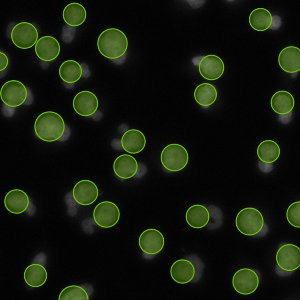
\includegraphics{drawables.jpg}}
\end{center}
\caption{\label{figure:drawables}
    Detected nuclei marked with semi-transparent circles drawn on the image using \code{DrawableCircle}: centers indicate detected object centers and radii -- object sizes
}
\end{figure}

\section*{Analysing RNAi screens}

Using \EBImage\ features described above, it is relatively straightforward to write an \R{} script for the automated analysis of images in the whole RNAi microscopy screen. Without going into biological details, we are interested in identification of nuclei and cells from images like in Figure \ref{figure:channels}, which are recorded for every RNAi target gene. We are particularly interested in the position, number, size, density and fluorescent intensity of these objects.

\EBImage\ provides a function called \code{objectCount}, which takes a distance map and identifies objects based on this distance map. It can also take the original image as a reference to calculate object intensities. In the current implementation, the algorithm sequentially searches through the distance map for the highest value, which is added as the position of a newly identified object. It then starts filling the distance map with the background color (black) in all directions, in which distance-map values decrease, until either the background is reached or the values start rising again (which indicates a neighboring object). Algorithm repeats until a newly found distance map value is smaller than the minimum object radius. The function returns a matrix with rows corresponding to identified objects and columns to their properties: index in the image stack, x and y coordinates, size, intensity (if applicable).

For every gene, the algorithm to implement (if simplified) looks as follows: load and normalize images, combine channels if required and renormalize, segment images, generate distance maps, use distance maps for objects counting, supply original images to the object counting function as references to detect object intensities, generate preview images with detected objects marked. The results of object detection can then be analyzed statistically to generate gene hit lists etc. This algorithm is illustrated in the following example code (which detects cells) and in Figure \ref{figure:analysis}. The source images as in Figure \ref{figure:channels}{\bf a}, {\bf b} and {\bf c} are denoted here as \code{src}.

\begin{verbatim}
> for (X in genes) {
+  files <- dir(pattern = X)
+  src <- read.image(files)
+  src <- normalize(src, independent = TRUE)
+  a <- normalize(abc[,,1] + sqrt(abc[,,3]))
+  b <- thresh(a, 100, 100, 0.04, TRUE)
+  C <- distMap(b)
+  res <- objectCount(C, src[,,3], 400)
+  d <- toRGB(a)
+  r <- sqrt(res[,4] / pi)
+  cx <- DrawableCircle(res[,2], res[,3], r)
+  d <- draw(d, cx)
+  resAll <- rbind(resAll, res)
+ }
> print(resAll)
      [,1] [,2] [,3] [,4]      [,5]
 [1,]    1   90  218 2012 339.86735
 [2,]    1  206   71 2041 374.20408
 ...
\end{verbatim}

\begin{figure}
\vspace*{.1in}
\begin{center}
\scalebox{1.0}{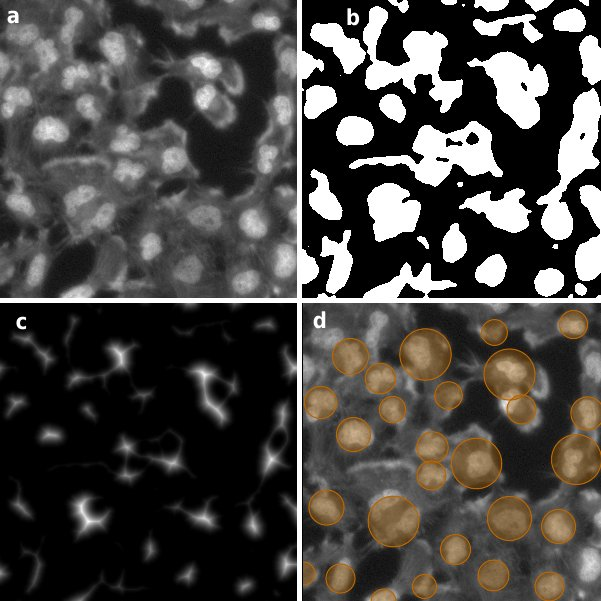
\includegraphics{analysis.jpg}}
\end{center}
\caption{\label{figure:analysis}
    Illustration of the object detection algorithm: (a) combined image of cells and nuclei (cellular image brightened by the {\em sqrt}), (b) image {\bf a} after blurring and thresholding, (c) normalized distance map generated from image {\bf b}. (d) detected cells marked by semi-transparent drawables
}
\end{figure}

Currently, the authors are working on a new version of \code{objectCount}, which is based on a modified {\em watershed algorithm}.

\begin{figure}
\vspace*{.1in}
%\begin{center}
\scalebox{0.5}{
\includegraphics{logo.jpg}}
%\end{center}
\end{figure}

\section*{Acknowledgements}

Authors would like to thank F.~Fuchs and M.~Boutros for experimental data, which existence and necessity to be analyzed caused the appearance of \EBImage; R.~Gottardo and F.~Swidan for testing the package on \lib{MacOS X}; the {\em BioConductor} project for hosting the software and the European Bioinformatics Institute (EBI), Cambridge, UK, for the financial support.

\begin{thebibliography}{1}
\expandafter\ifx\csname natexlab\endcsname\relax\def\natexlab#1{#1}\fi
\expandafter\ifx\csname url\endcsname\relax
  \def\url#1{{\tt #1}}\fi

\bibitem[Carpenter et al.(in preparation)]{R:Carpenter:prep}
    A.~E.~Carpenter, T.~R.~Jones, M.~Lamprecht, D.~B.~Wheeler, C.~Clarke, I.~H.~Kang, O.~Friman, D.~A.~Guertin, J.~H.~Chang, R.~Lindquist, J.~Moffat, P.~Golland, and D.~M.~Sabatini.
    \newblock CellProfiler: image analysis for high throughput microscopy.
    \newblock {\em In preparation}.
    \newblock URL \url{http://www.cellprofiler.org/}

\bibitem[Fuchs and Boutros(2006)]{R:Fuchs+Boutros:2006}
    F.~Fuchs and M.~Boutros.
    \newblock Cellular phenotyping by RNAi.
    \newblock {\em Brief Funct Genomic Proteomic.}, 5:52--56, 2006.

\bibitem[ImageMagick(1999)]{R:ImageMagick:1999}
    ImageMagick: Software to convert, edit, and compose images.
    \newblock {\em Copyright: ImageMagick Studio LLC}, 1999-2006.
    \newblock URL \url{http://www.imagemagick.org/}

\bibitem[Lotufo and Zampirolli(2001)]{R:Lotufo+Zampirolli:2001}
    R.~Lotufo and F.~Zampirolli.
    \newblock Fast Multidimensional Parallel Euclidean Distance Transform Based on Mathematical Morphology.
    \newblock {\em SIBGRAPI-2001/Brazil}, 100--105, 2001 (conference proceedings).

\bibitem[Neumann et al.(2006)]{R:Neumann:2006}
    B.~Neumann, M.~Held, U.~Liebel, H.~Erfle, P.~Rogers, R.~Pepperkok and J.~Ellenberg.
    \newblock High-throughput RNAi screening by time-lapse imaging of live human cells.
    \newblock {\em Nature Mathods}, 3\penalty0 (5):\penalty0 385--390, 2006.

\bibitem[SIP Toolbox(2005)]{R:SIP:2005}
    SIP Toolbox: Scilab Image Processing Toolbox.
    \newblock {\em Sourceforge}, 2005.
    \newblock URL \url{http://siptoolbox.sourceforge.net/}

\end{thebibliography}
